\section{Числовые характеристики случайных величин: моменты, математическое ожидание, дисперсия. Их свойства}

\subsubsection{Математическое ожидание случайной величины}

\begin{defn}
    Пусть задано вероятностное пространство $(\Omega, \mathcal{F}, \mathbb{P})$ и случайная величина $\xi \colon \Omega \mapsto \mathbb{R}$. 
    Если существует интеграл Лебега от $\xi$ по мере $\mathbb{P}$ по множеству $\Omega$, то он называется \textit{математическим ожиданием} случайной величины $\xi$ и обозначается как $\mathbb{E}\xi$ или $\operatorname{M} \! \xi$.
    \begin{equation*}
        \mathbb{E}\xi = \int\limits_{\Omega} \xi(\omega) \mathbb{P}(d\omega).
    \end{equation*}
\end{defn}

\begin{defn}
    \textit{Математическое ожидание (среднее значение, первый момент)} случайной величины $\xi$, 
    имеющей дискретное распределение со значениями $a_1, a_2, \ldots$~--- сумма абсолютно\footnote{Согласно теореме Римана из математического анализа, члены условно сходящегося ряда можно переставить так, что он будет сходиться к любому наперёд заданному числу. 
        Таким образом, если допустить условную сходимость, то математическое ожидание \sout{goes brrr} зависит от способа вычисления.} 
    сходящегося ряда.
    \begin{equation*}
        \mathbb{E} \xi=\sum\limits_{i} a_{i} p_{i}=\sum\limits_{i} a_{i} \mathbb{P}(\xi=a_{i}).
    \end{equation*}
\end{defn}

\begin{defn}
    \textit{Математическое ожидание} случайной величины $\xi$, имеющей абсолютно непрерывное распределение с плотностью распределения $f(x)$~--- значение абсолютно сходящегося интеграла
    \begin{equation*}
        \mathbb{E} \xi=\int\limits_{\mathbb{R}} x \, f(x) \, dx.
    \end{equation*}
\end{defn}

Математическое ожидание имеет простой физический смысл: если на прямой разместить единичную массу, поместив в точки $a_i$ массу $p_i$ (для дискретного распределения) или «размазав» её с плотностью $f_\xi(x)$ (для абсолютно непрерывного распределения), то точка $\mathbb{E}\xi$ будет координатой <<центра тяжести>> прямой.

\begin{namedthm}[Свойства математического ожидания]
    Везде далее предполагается, что рассматриваемые математические ожидания существуют.
\begin{enumerate}
    \item 
        Для произвольной борелевской функции $g(x)$ со значениями в $\mathbb{R}$:
        \begin{equation*}
        \mathbb{E} g(\xi) =
        \begin{cases}
            \sum\limits_{k} g\left(a_{k}\right) \mathbb{P}\left(\xi=a_{k}\right), & \text {если~} P_{\xi} \text {~дискретно}; \\
            \int\limits_{-\infty}^{+\infty} g(x) f_{\xi}(x) \, dx, & \text {если~} P_{\xi} \text{~абсолютно непрерывно.}
        \end{cases}
        \end{equation*}

        Такое же свойство верно и для числовых функций нескольких аргументов $g(x_1, \ldots, x_n)$, если $\xi$~--- вектор из $n$ случайных величин, а в сумме и в интеграле участвует их совместное распределение. Например, для $g(x,y) = x + y$ и для случайных величин $\xi$ и $\eta$ с плотностью совместного распределения $f(x,y)$ верно: 
        \begin{equation}
            \label{expectation_of_sum}
            \mathbb{E}(\xi+\eta)=\int\limits_{-\infty}^{\infty} \int\limits_{-\infty}^{\infty}(x+y) f(x, y) d x d y;
        \end{equation}
    \item 
        Математическое ожидание линейно:
        \begin{equation*}
            \mathbb{E}(a \xi + b) = a \mathbb{E}\xi + b \quad \forall a,b \in \mathbb{R};
        \end{equation*}
    \item
        $\mathbb{E}(\xi + \eta) = \mathbb{E}\xi + \mathbb{E}\eta$;
    
    \item 
        Если $\xi \overset{\text{п.н.}}{\geqslant} 0$, то $\mathbb{E}\xi \geqslant 0$;
    
        \textbf{Следствие.}
        \begin{compactlist}
            \item Если $\xi \overset{\text{п.н.}}{\leqslant} \eta$, то $\mathbb{E}\xi \leqslant \mathbb{E}\eta$;
            \item Если $a \overset{\text{п.н.}}{\leqslant} \xi \overset{\text{п.н.}}{\leqslant} b$, то $a \leqslant \mathbb{E}\xi \leqslant b$.
        \end{compactlist}
    
    \item 
        Если $\xi$ и $\eta$~--- независимые случайные величины, то $\mathbb{E}(\xi \eta) = \mathbb{E}\xi \, \mathbb{E}\eta$;
        
        \textbf{Замечание.}
        Обратное, вообще говоря, \hyperlink{counter_exmp_independence}{неверно}.
    \item 
        $\left| \mathbb{E}\xi \right| \leqslant \mathbb{E}|\xi|$;
    
    \item 
        $\xi \overset{\text{п.н.}}{\geqslant} 0, \: \mathbb{E}\xi = 0 \; \Rightarrow \; \xi \overset{\text{п.н.}}{=} 0$;
    
    \item 
        $\myprob{A} = \mathbb{E}\bigl( \mathrm{I}_A(\omega) \bigr)$, где $\mathrm{I}_A(\omega)$~--- индикатор:
        \begin{equation*}
            \mathrm{I}_A(\omega) = \mathrm{I}(\omega \in A) =
            \begin{cases}
            1, & \omega \in A \\
            0, & \text{иначе};
            \end{cases}
        \end{equation*}
        
    \item 
        Если функция $g(x)$ выпукла, то $\mathbb{E}g(\xi) \geqslant g(\mathbb{E}\xi)$ (неравенство Йенсена).
    
\end{enumerate}
\end{namedthm}

\begin{proof}
\begin{enumerate}
    \item 
        Достаточно рассмотреть случайную величину $\eta = g(\xi)$ на том же вероятностном пространстве и заметить, что $\forall \, \omega \in \Omega \colon \eta(\omega) = g(\xi(\omega))$. 
        Тогда 
        $$ \mathbb{E}\eta = \int\limits_{\Omega} \eta(\omega) \mathbb{P}(d\omega) = \int\limits_{\Omega} g(\xi(\omega)) \mathbb{P}(d\omega). $$
        Отсюда и вытекают формулы для дискретного и абсолютного случая.
        
    \item 
        Рассмотрим функцию $g(x) \equiv ax + b$ и произвольную случайную величину $\xi$. Тогда 
        \begin{multline*}
            \mathbb{E}(a \xi + b) 
            = \mathbb{E}g(\xi) 
            = \int\limits_{\Omega}g(\xi(\omega))\mathbb{P}(d\omega)
            = a \int\limits_{\Omega}\xi(\omega)\mathbb{P}(d\omega) + b \int\limits_{\Omega}\mathbb{P}(d\omega) = \\
            = a \, \mathbb{E}\xi + b \, \myprob{\Omega} 
            = a \, \mathbb{E}\xi + b.
        \end{multline*}
        
    \item 
        Воспользуемся равенством \eqref{expectation_of_sum} и теоремой о совместном распределении:
        $$\begin{aligned}
            \mathbb{E}(\xi+\eta) &=\int\limits_{-\infty}^{\infty} \int\limits_{-\infty}^{\infty}(x+y) f(x, y) \, dx dy=\\
            &=\int\limits_{-\infty}^{\infty} x \, dx \int\limits_{-\infty}^{\infty} f(x, y) \, dy + \int\limits_{-\infty}^{\infty} y \, dy \int\limits_{-\infty}^{\infty} f(x, y) \, dx=\\
            &=\int\limits_{-\infty}^{\infty} x f_{\xi}(x) \, dx + \int\limits_{-\infty}^{\infty} y f_{\eta}(y) \, dy=\mathbb{E} \xi+\mathbb{E} \eta.
        \end{aligned}$$
    \item 
        Неотрицательность $\xi$ означает, что $a_i \geqslant 0$ при всех $i \colon p_i > 0$ в случае дискретного распределения, либо $f_\xi(x) = 0$ при $x < 0$ (кроме, может быть, множества меры нуль) - для абсолютно непрерывного распределения. 
        И в том, и в другом случае имеем:
        $$\mathbb{E} \xi=\sum a_{i} p_{i} \geqslant 0 \quad \text {или} \quad \mathbb{E} \xi=\int\limits_{0}^{\infty} x f(x) \, dx \geqslant 0.$$
        
    \item 
        В равенстве (1) заменим сложение умножением и плотность совместного распределения произведением плотностей (это возможно в силу независимости случайных величин):
        $$\begin{aligned}
            \mathbb{E}(\xi \eta) &=\int\limits_{-\infty}^{\infty} \int\limits_{-\infty}^{\infty} x y f_{\xi}(x) f_{\eta}(y) \,  dx dy = \\
            &=\int\limits_{-\infty}^{\infty} x f_{\xi}(x) \, dx \int\limits_{-\infty}^{\infty} y f_{\eta}(y) \, dy = \mathbb{E} \xi \mathbb{E} \eta.
        \end{aligned}$$
        
    \item 
        Это верно в силу неравенства треугольника (для дискретного случая) и аналогичного неравенства для интегралов (для непрерывного случая).
    
    \item 
        %Это свойство мы докажем, заранее предполагая, что $\xi$ имеет дискретное распределение с неотрицательными значениями $a_k \geqslant 0$. 
        \begin{itemize}
            \item Дискретный случай:

                Учитывая то, что $a_k \geqslant 0$, равенство $\mathbb{E}\xi = \sum a_k p_k = 0$ означает, что все слагаемые в этой сумме равны нулю, т. е. все вероятности $p_k$ нулевые, кроме вероятности, соответствующей значению $a_k = 0$.
            \item Абсолютно непрерывный случай:
                
                Условие $\xi \overset{\text{п.н.}}{\geqslant} 0$ говорит о том, что при $x < 0$ плотность равна нулю всюду, кроме, может быть, множества меры нуль по Лебегу.
                В самом деле, если существует борелевское множество $B \subset \{x \: | \: x < 0\}$ ненулевой меры и при этом ${f_{\xi}(x) > 0 \; \forall \, x \in B}$, 
                то ${\mathbb{P}\left(\xi \in B\right) = \int\limits_{B} f_{\xi}(x) \, dx > 0}$, т.е. случайная величина принимает отрицательные значения с ненулевой вероятностью, что противоречит ограничению.
                Учитывая это, можем написать
                $$ \mathbb{E}\xi = \int\limits_{-\infty}^{+\infty} x f_{\xi}(x) \, dx = \int\limits_{0}^{+\infty} x f_{\xi}(x) \, dx \geqslant 0,$$
                так как на промежутке интегрирования $x \geqslant 0$, а плотность по определению неотрицательна.
        \end{itemize}
    \item 
        Следует непосредственно из определений индикатора и матожидания.
    
    \item 
        Начнём с утверждения: если функция $g$ выпукла, то для любого ${y \in \mathbb{R}} \; {\exists \: c = c(y) \colon} \forall \: x \in \mathbb{R} \; g(x) \geqslant g(y) + c(y)(x - y)$. 
        Это вытекает из того, что график выпуклой функции лежит не ниже любой из касательной к нему.\footnote{Вообще говоря, выпуклая функция может не иметь первой производной и, следовательно, касательной на не более чем счётном множестве точек, но тогда можно заменить касательную на опорную гиперплоскость.} 
        Положим в этом неравенстве $y = \mathbb{E}\xi$. 
        Тогда
        $$ g(\xi) \geqslant g(\mathbb{E}\xi) + c(\mathbb{E}\xi)(\xi - \mathbb{E}\xi) $$
        $$ \mathbb{E}g(\xi) \geqslant \mathbb{E}g(\mathbb{E}\xi) +  \mathbb{E}c(\mathbb{E}\xi)(\xi - \mathbb{E}\xi)$$
        Здесь $g(\mathbb{E}\xi), c(\mathbb{E}\xi)$ - константы, а $\mathbb{E}(\xi - \mathbb{E}\xi) = 0$, а значит,
        $$ \mathbb{E}g(\xi) \geqslant g(\mathbb{E}\xi).$$
\end{enumerate}
\end{proof}

\subsubsection{Дисперсия и моменты старших порядков}

\begin{defn}
    Пусть ${\mathbb{E}|\xi|^k < \infty}$. 
    \begin{enumerate}
        \item 
            ${\mathbb{E}\xi^k}$~--- \textit{момент порядка $k$ или $k$-й момент} случайной величины $\xi$;
        \item 
            ${\mathbb{E}|\xi|^k}$~--- \textit{абсолютный $k$-й момент};
        \item 
            $\mu_k = {\mathbb{E}(\xi - \mathbb{E}\xi)^k}$~--- \textit{центральный $k$-й момент};
        \item 
            ${\mathbb{E}|\xi - \mathbb{E}\xi|^k}$~--- \textit{абсолютный центральный $k$-й момент} случайной величины $\xi$
    \end{enumerate}
\end{defn}

\begin{defn}
    Число $\mathbb{D}\xi = \mathbb{E}(\xi - \mathbb{E}\xi)^2$ (центральный момент второго порядка) называется \textit{дисперсией} случайной величины $\xi$, $\sigma = \sqrt{\mathbb{D}\xi}$~--- её \textit{среднеквадратичным отклонением}.
\end{defn} 

\begin{thm*}
    Если существует момент порядка $t > 0$ случайной величины $\xi$, то существует и ее момент порядка $s$, где $0 < s < t$.
\end{thm*}

\begin{proof} 
Заметим, что $|\xi|^s \leqslant |\xi|^t + 1.$ 
В силу следствия из свойства 4 для математического ожидания можно получить из неравенства для случайных величин такое же неравенство для их математических ожиданий: $\mathbb{E}|\xi|^s \leqslant \mathbb{E}|\xi|^t + 1 < \infty.$
\end{proof}

\subsubsection{Свойства дисперсии}

\begin{rmrk}
    Во всех свойствах предполагается существование вторых моментов случайных величин. 
    Тогда (в силу вышеописанной теоремы) существуют и сами матожидания.
\end{rmrk} 

\begin{enumerate}

    \item 
        Дисперсия может быть вычислена по формуле: $\mathbb{D}\xi = \mathbb{E}\xi^2 - (\mathbb{E}\xi)^2$.
    
        \begin{proof}
            Обозначим для удобства $a = \mathbb{E}\xi.$ Тогда
        $$\mathbb{D} \xi=\mathbb{E}(\xi-a)^{2}=\mathbb{E}\left(\xi^{2}-2 a \xi+a^{2}\right)=\mathbb{E} \xi^{2}-2 a \mathbb{E} \xi+a^{2}=\mathbb{E} \xi^{2}-a^{2}.$$
        \end{proof} 
    
    \item 
        При умножении случайной величины на постоянную $c$ дисперсия увеличивается в $c^2$ раз: $\mathbb{D}(c\xi) = c^2\mathbb{D}\xi.$
    \item 
        Дисперсия всегда неотрицательна: $\mathbb{D}\xi \geqslant 0.$
    
        \begin{proof}
            Пусть $a = \mathbb{E}\xi.$ Дисперсия есть математическое ожидание неотрицательной случайной величины $(\xi - a)^2$, откуда (и из свойства 5 матожидания) следует неотрицательность дисперсии.
        \end{proof}
    
    \item 
        Дисперсия обращается в нуль лишь для вырожденного распределения: если $\mathbb{D}\xi = 0$, то $\xi \overset{\text{п.н.}}{=} \text{const}$, и наоборот.
    
        \begin{proof}
            $\mathbb{D}\xi = 0 \Rightarrow (\xi - a)^2 \overset{\text{п.н.}}{=} 0, \, \xi \overset{\text{п.н.}}{=} a =\text{const}$. И наоборот: если $\xi \overset{\text{п.н.}}{=} c$, то $\mathbb{D} \xi=\mathbb{E}(c-\mathbb{E} c)^{2}=\mathbb{E} \, 0=0.$
        \end{proof} 
    
    \item 
        Дисперсия не зависит от сдвига случайной величины на постоянную: $\mathbb{D}(\xi + c) = \mathbb{D}\xi.$
    
    \item 
        Если $\xi$ и $\eta$ независимы, то $\mathbb{D}(\xi + \eta) = \mathbb{D}\xi + \mathbb{D}\eta.$
    
        \begin{proof}
        Действительно, применяя свойство (5) матожидания, получим:
        $$\begin{aligned}
        \mathbb{D}(\xi+\eta) &=\mathbb{E}(\xi+\eta)^{2}-(\mathbb{E}(\xi+\eta))^{2}=\\
        &=\mathbb{E} \xi^{2}+\mathbb{E} \eta^{2}+2 \mathbb{E}(\xi \eta)-(\mathbb{E} \xi)^{2}-(\mathbb{E} \eta)^{2}-2 \mathbb{E} \xi \, \mathbb{E} \eta=\mathbb{D} \xi+\mathbb{D} \eta
        \end{aligned}.$$
        \end{proof}
        
        \begin{rmrk}
            Обратное, аналогично замечанию к свойству (5) матожидания, \hyperlink{counter_exmp_independence}{неверно}.
        \end{rmrk} 
        
        \begin{crlr}
            Если $\xi$ и $\eta$ независимы, то $\mathbb{D}(\xi-\eta)=\mathbb{D} \xi+\mathbb{D} \eta$. 
        \end{crlr} 
        
        \begin{proof}
            Из свойств (6) и (2) получим: 
            $$\mathbb{D}(\xi-\eta)=\mathbb{D}(\xi+(-\eta))=\mathbb{D} \xi+\mathbb{D}(-\eta)=\mathbb{D} \xi+(-1)^{2} \mathbb{D} \eta=\mathbb{D} \xi+\mathbb{D} \eta.$$
        \end{proof} 
        
        \begin{crlr}
            Для произвольных случайных величин $\xi$ и $\eta$ имеет место равенство:
            $$\mathbb{D}(\xi \pm \eta)=\mathbb{D} \xi+\mathbb{D} \eta \pm 2(\mathbb{E}(\xi \eta)-\mathbb{E} \xi\, \mathbb{E} \eta).$$
        \end{crlr} 
    
        \begin{rmrk}
        В последнем равенстве величина $\mathbb{E}(\xi \eta)-\mathbb{E} \xi \, \mathbb{E} \eta$ есть \textit{ковариация} случайных величин $\xi$ и $\eta$~--- $\text{cov}(\xi, \eta)$.
        \end{rmrk}
    
\end{enumerate}

\subsubsection{Прочие числовые характеристики}
    \definecolor{color1}{HTML}{ffba00}
    \definecolor{color2}{HTML}{00bfff}
    \definecolor{color3}{HTML}{ff00ff}
    \pgfplotsset{skewkurt/.style={
        height=10cm, width=10cm,
        xmin=-1, xmax=7,
        ymin=-0.05,
        ymax=0.7,
        ticks=none,
        axis line style = thick,
        axis lines = middle,
        enlargelimits=false,
   }}
    \tikzset{
        declare function={normal(\x,\sstd,\mu)=1/sqrt(2*pi*\sstd)*exp(-(\x-\mu)^2/(2*\sstd));},
        declare function={
            cdfapp(\x)=1/(1 + exp(-0.07056*(\x)^3 - 1.5976*(\x);
       },
        declare function={
            sknorm(\x,\mu,\std,\alpha)=
            2 * normal(\x,\std*\std,\mu) * 
            cdfapp(\alpha*(\x-\mu)/\std);
       },
   }
\begin{defn}
    \textit{Коэффициент асимметрии} случайной величины $\xi$:
    \begin{equation*}
        \gamma_1=\mathbb{E}\left(\frac{\xi - \mathbb{E}\xi}{\sqrt{\mathbb{D}\xi}}\right)^3 = \frac{\mu^3}{\sigma^3}
    \end{equation*}
    Характеризует <<скошенность>> графика плотности распределения: \medskip\hfill\break
    \begin{center}
    \begin{tikzpicture}
    \begin{axis}[skewkurt, ymax=0.5]
        \draw [dashed,black!50] (3,0) -- (3,0.4);
        \addplot[very thick, color1, samples=100,domain=-1:7] {sknorm(x,3,1.9,-8)};
        \addlegendentry{$\gamma_1<0$}
        \addplot[very thick, color2, samples=100,domain=-1:7] {sknorm(x,3,1.9,8)};
        \addlegendentry{$\gamma_1>0$}
        \addplot[very thick, color3, samples=100,domain=-1:7] {sknorm(x,3,1,0)};
        \addlegendentry{$\gamma_1=0$}
    \end{axis}
    \end{tikzpicture}
    \end{center}
\end{defn}

\begin{defn}
    \textit{Коэффициент эксцесса} случайной величины $\xi$:
    \begin{equation*}
        \gamma_2=\mathbb{E}\left(\frac{\xi - \mathbb{E}\xi}{\sqrt{\mathbb{D}\xi}}\right)^4 - 3 = \frac{\mu^4}{\sigma^4} - 3
    \end{equation*}
    Характеризует <<островершинность>> графика плотности распределения:
    \medskip\hfill\break
    \begin{center}
    \begin{tikzpicture}
    \begin{axis}[skewkurt]
        \draw [dashed,black!50] (3,0) -- (3,0.625);
        \addplot[very thick, color1, samples=100,domain=-1:7] {normal(x,2.2,3)};
        \addlegendentry{$\gamma_2<0$}
        \addplot[very thick, color2, samples=100,domain=-1:7] {normal(x,0.4,3)};
        \addlegendentry{$\gamma_2>0$}
        \addplot[very thick, color3, samples=100,domain=-1:7] {normal(x,1,3)};
        \addlegendentry{$\gamma_2=0$}
    \end{axis}
    \end{tikzpicture}
    \end{center}
\end{defn}

\begin{rmrk}
    Слагаемое $-3$ добавлено, чтобы коэффициент эксцесса стандартного нормального распределения был равен нулю. Иногда его не учитывают и считают, что коэффициент эксцесса $\mathrm{N}(0,1)$ равен 3.
\end{rmrk}

\iffalse
\medskip\hfill\break
    \begin{center}
    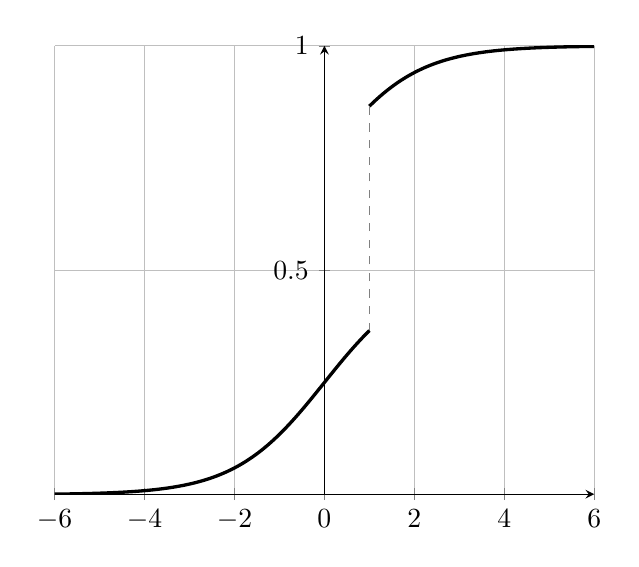
\begin{tikzpicture}[declare function={sigma(\x)=1/(1+exp(-\x));}]
\begin{axis}
[
    grid=major,     
    xmin=-6,
    xmax=6,
    axis x line=bottom,
    ytick={0,.5,1},
    ymax=1,
    axis y line=middle,
    samples=100,
    domain=-6:6,
    legend style={at={(1,0.9)}}     
]
    \draw [dashed,black!50] (1,0.365) -- (1,0.865);
    \addplot[very thick,black,mark=none, samples=100,domain=-6:1]   (x, {.5 * sigma(x)});
    \addplot[very thick,black,mark=none, samples=100,domain=1:6]   (x, {.5 + .5 * sigma(x)});
\end{axis}
\end{tikzpicture}
    \end{center}
\fi
